
\chapter{C4 Level 3 - Components}
\label{appendix:design:architecture:platform:components}

The component level describes the internals of a specific container. A container is made up of a number of components, each with well-defined responsibilities. In the following diagrams the dependencies between the various components will also be presented.

Most developed containers share the same architecture and will therefore be addressed as groups of containers.

The physical view will not be presented since all relevant details have been addressed above.

\section{Components Level - Logical View}
\label{par:design:architecture:platform:components:logical}

The architectures used in the various developed containers can be condensate into 3 types with minor variations:

\begin{itemize}
   \item \textbf{Frontend Architecture}: used on all Configuration scope frontend containers;
   \item \textbf{Configuration Backend Architecture}: used on all Configuration scope backend containers;
   \item \textbf{Data Flow Architecture}: used on most Data Flow scope containers.
\end{itemize}

Starting with the Frontend Architecture used, it was decided to maintain two distinct domains (Model and DTOS) in order to meet the \gls{SRP} (high cohesion) and to lower the coupling between the information displayed in the UI and the data sent/received by the container. This segmentation led to the addition of the Mapper component, which has the responsibility of converting the data (DTOS component) into information (Model component) and vice-versa. The Auth component indicates what backend resources the user has access to, by decoding the \textit{access token}, and the Utils component has several methods commonly used to process backend requests. These two components are reused in all frontend containers, including the ones related to the Business Applications.

As an example, the logical view of the Data Decoder Frontend is presented in Figure~\ref{fig:design:architecture:platform:component:logical:diagram:decoder}.

\begin{figure}[H]
   \centering
   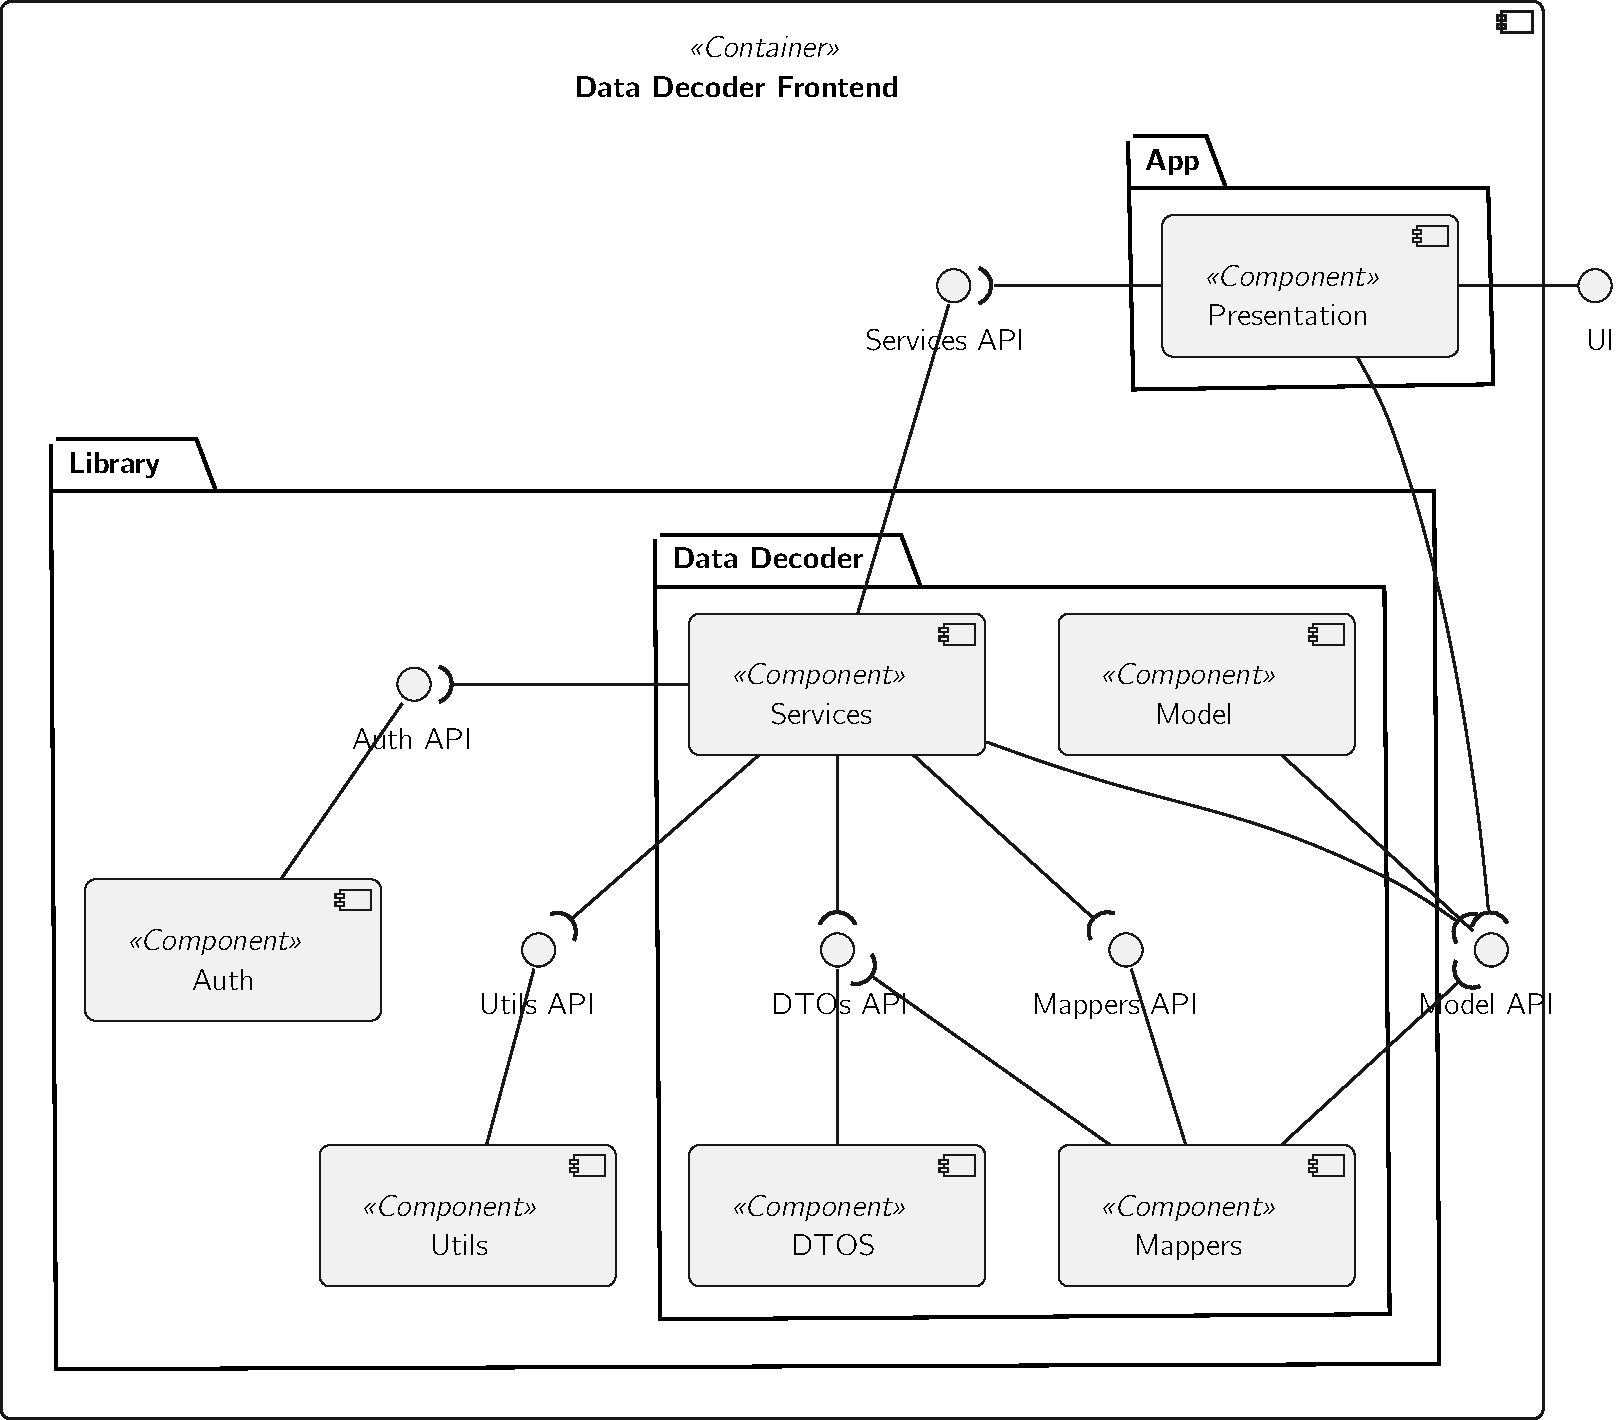
\includegraphics[page=1,width=0.7\columnwidth]{assets/diagrams/design/architectural/level3/logical/data-decoder-frontend.pdf}
   \caption[Data Decoder Frontend - Component Level - Logical View Diagram]{Data Decoder Frontend - Component Level - Logical View Diagram}
   \label{fig:design:architecture:platform:component:logical:diagram:decoder}
\end{figure}

This architecture is used on the containers: (i) Device Management Frontend, (ii) Data Decoder Frontend, (iii) Data Processor Frontend, (iv) Rule Management Frontend. The UI Aggregator has a simpler architecture them the other frontend containers, it is comprised by a Presentation component that depends on the Auth component to handle user authentication and authorization.

Next, the Configuration Backend Architecture is discussed. It is based on the Onion Architecture, an architecture pattern that ``emphasizes separation of concerns throughout the system'' and ``leads to more maintainable applications'' \parencite{onion}.

As an example the logical view of the Device Management Backend is presented in Figure~\ref{fig:design:architecture:platform:component:logical:diagram:device}.

\begin{figure}[H]
   \centering
   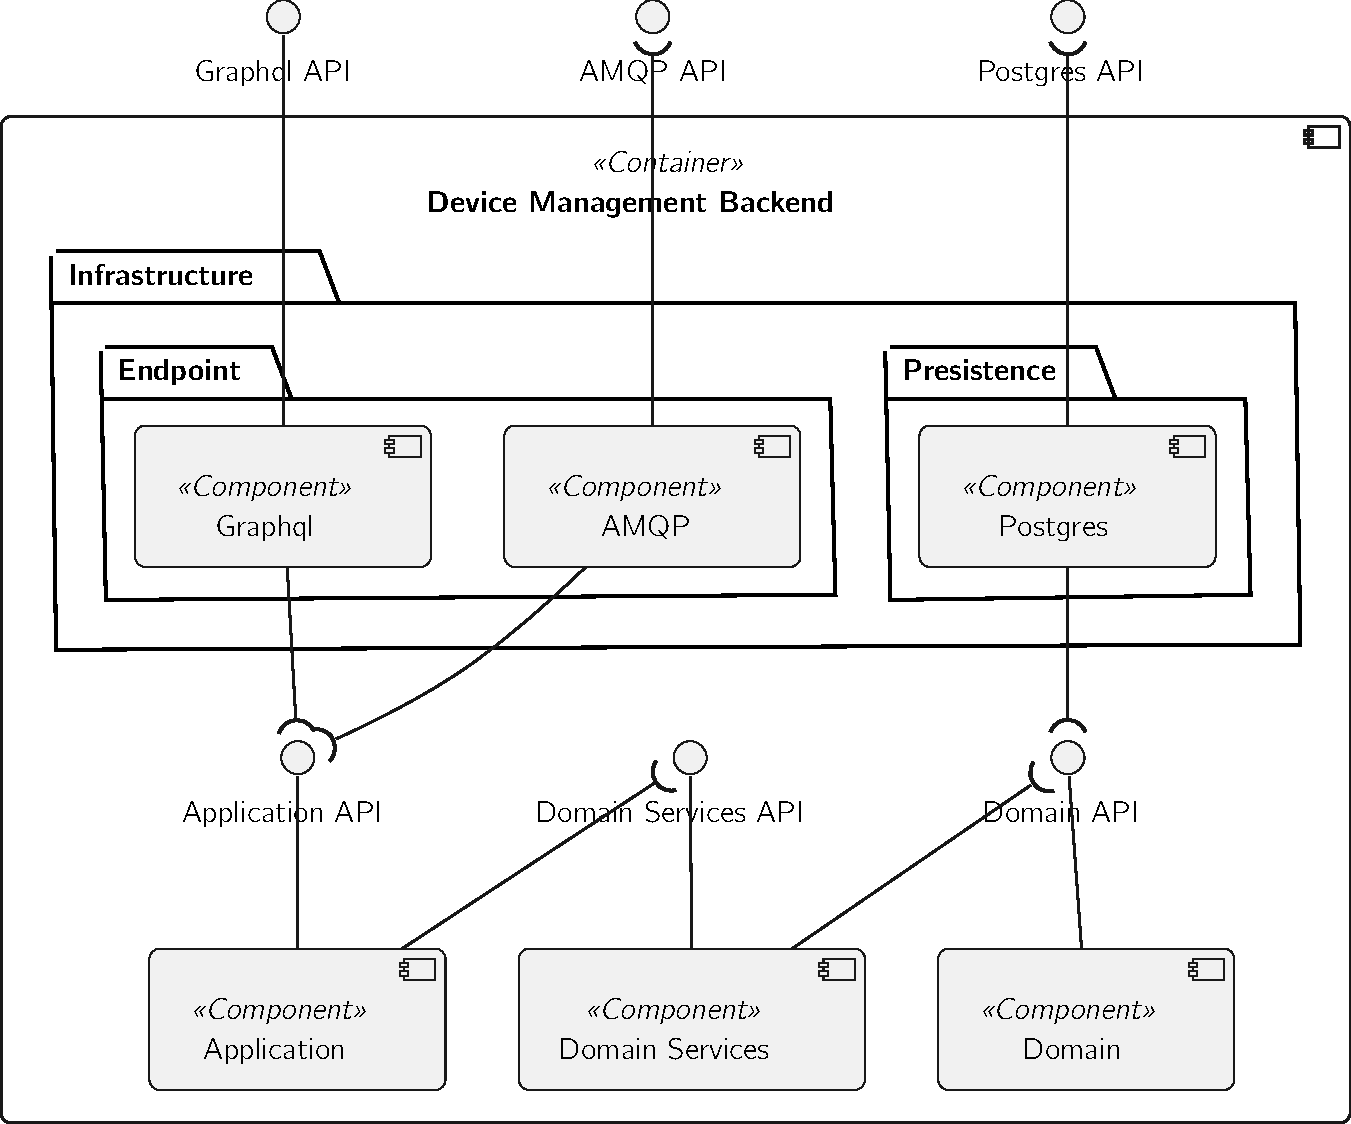
\includegraphics[page=1,width=0.8\columnwidth]{assets/diagrams/design/architectural/level3/logical/device-management-backend.pdf}
   \caption[Device Management Backend - Component Level - Logical View Diagram]{Device Management Backend - Component Level - Logical View Diagram}
   \label{fig:design:architecture:platform:component:logical:diagram:device}
\end{figure}

This architecture is used on the containers: (i) Device Management Backend, (ii) Data Decoder Backend, (iii) Data Processor Backend, (iv) Rule Management Backend, (v) Identity Management Backend.

The following table, Table~\ref{tab:design:architecture:platform:components:logical:backend}, discusses each component responsibilities.

\begin{table}[H]
   \centering
   \caption{Configuration Backend components responsibilities}
   \label{tab:design:architecture:platform:components:logical:backend}
   \begin{tabular}{@{}cl@{}}
   \toprule
   \textbf{Component}               & \textbf{Responsibilities}                                            \\ \midrule
   Infrastructure &
     \begin{tabular}[c]{@{}l@{}}- Enclose components that manage the Input/Output\\ operations required by the container.\end{tabular} \\ \midrule
   Endpoint &
     \begin{tabular}[c]{@{}l@{}}- Enclose components that are used by external\\ containers to interact with the container.\end{tabular} \\ \midrule
   \multirow{2}{*}{AMQP} &
     - Define how to consume and publish events in the Message Broker; \\
    &
     \begin{tabular}[c]{@{}l@{}}- Delegate the handling of events received to \\ specific Application processes.\end{tabular} \\ \midrule
   \multirow{2}{*}{GraphQl}         &
     \begin{tabular}[c]{@{}l@{}} - Define the interface to be consumed by the \\ frontend and external Systems;  \end{tabular} \\
                                    & - Delegate external requests made to specific Application processes.\\ \midrule
   Persistence &
     \begin{tabular}[c]{@{}l@{}}- Enclose components that interface with \\ containers responsible for persisting data.\end{tabular} \\ \midrule
   Postgres                         & - Interact with a database to persist and query data.                \\ \midrule
   \multirow{4}{*}{Application}     & - Represent the application processes;                               \\
    &
     \begin{tabular}[c]{@{}l@{}}- Ensure the propagation of events related to the\\ process in question, requiring this responsibility to AMQP;\end{tabular} \\
    &
     \begin{tabular}[c]{@{}l@{}}- Ensure the execution of the process in question,\\ requiring this responsibility to Domain Services;\end{tabular} \\
                                    & - Enforce user authorization.                                        \\ \midrule
   \multirow{3}{*}{Domain Services} & - Represent business processes;                                      \\
                                    & - Interact with the Domain;                                  \\
    &
     \begin{tabular}[c]{@{}l@{}}- Ensure the persistence of the data in question,\\ requiring this responsibility to the Persistence.\end{tabular} \\ \midrule
   \multirow{2}{*}{Domain}          & - Represent de business rules and concepts;                          \\
                                    & - Manage the system information.                                    \\ \bottomrule
   \end{tabular}
\end{table}

Finally the architecture used in containers related to the Data Flow Scope is presented. It is based on a simplified version of the Onion Architecture since the intrinsic processes of these containers are much simpler.

As an example the logical view of the Device Ownership Backend is presented in Figure~\ref{fig:design:architecture:platform:component:logical:diagram:ownership}.

\begin{figure}[H]
   \centering
   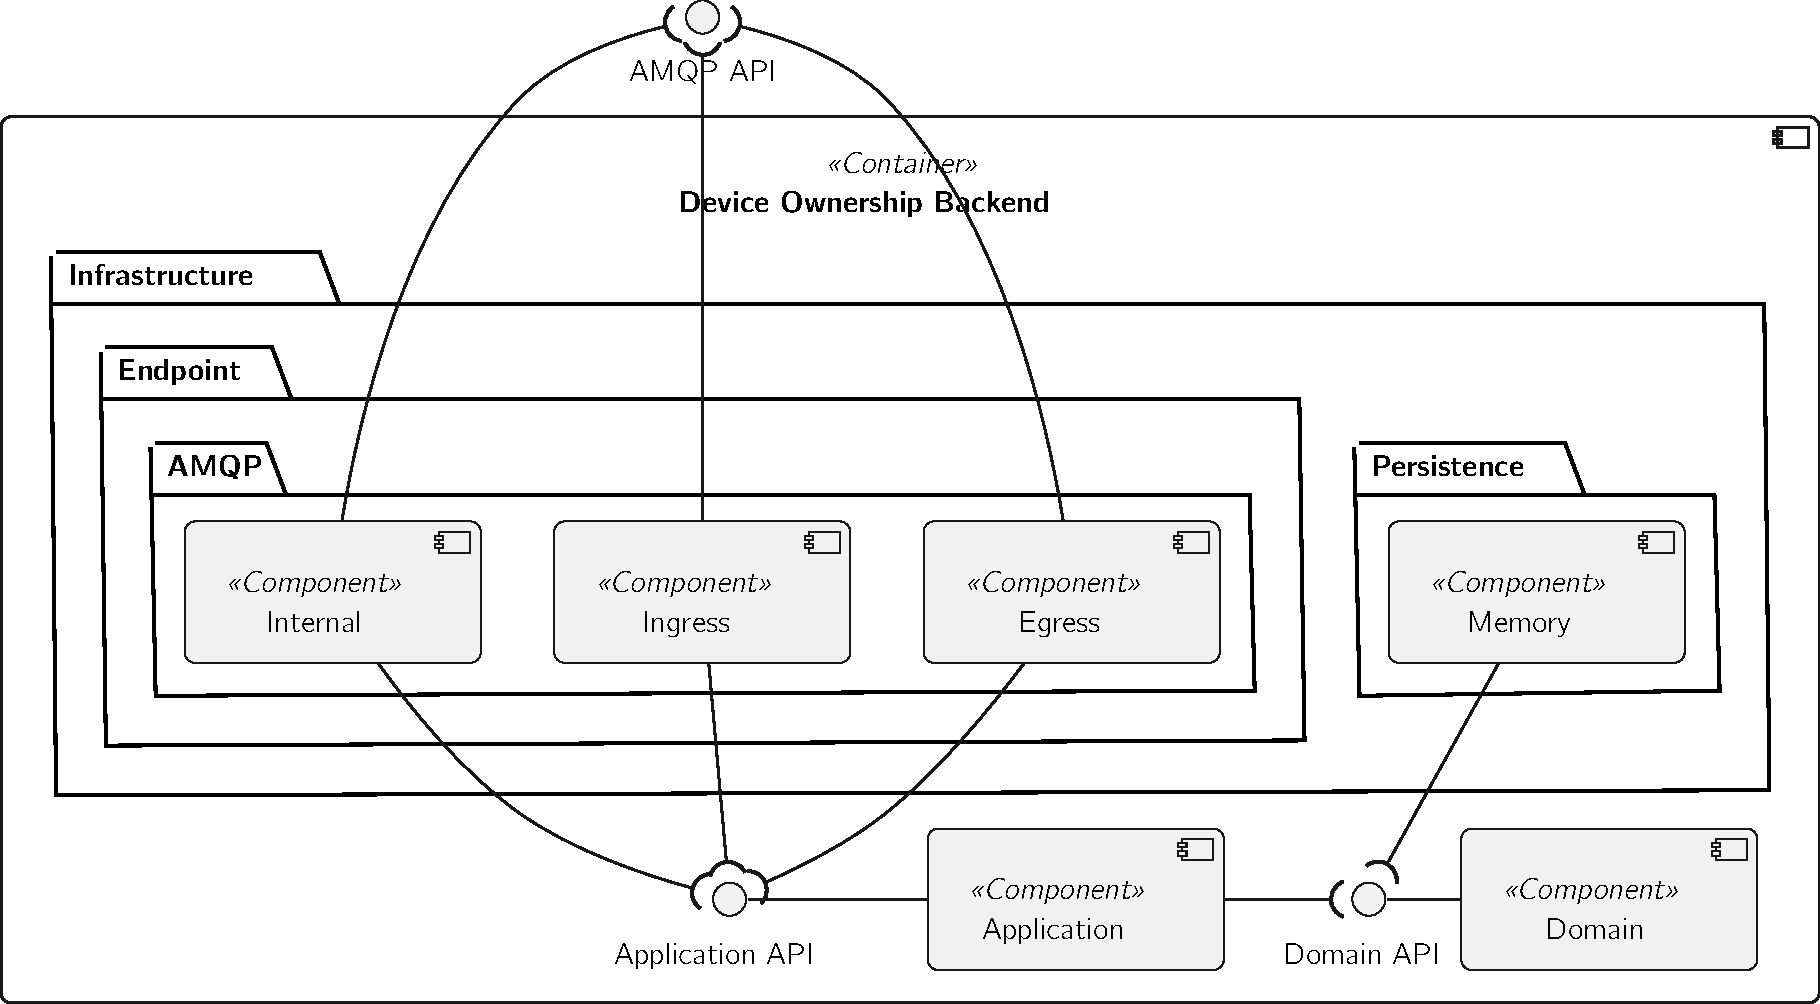
\includegraphics[page=1,width=\columnwidth]{assets/diagrams/design/architectural/level3/logical/device-ownership-backend.pdf}
   \caption[Device Ownership Backend - Component Level - Logical View Diagram]{Device Ownership Backend - Component Level - Logical View Diagram}
   \label{fig:design:architecture:platform:component:logical:diagram:ownership}
\end{figure}

This architecture is used on the containers: (i) Device Management Flow Backend, (ii) Data Decoder Flow Backend, (iii) Data Processor Flow Backend, (iv) Device Ownership Backend. The responsibilities of the components inside AMQP are:

\begin{itemize}
   \item Internal: responsible for communicating with the system via internal topic;
   \item Ingress: responsible for consuming events/messages coming from data, alert or command topics;
   \item Egress: responsible for publishing events/messages to the data or alert topics.
\end{itemize}

The Memory component is responsible for caching unhandled data units and other information relevant for each context. This component is not present in Data Validator Backend and Alert Dispatcher Backend since they don't need to store context information to function.

The Data Gateway, Device Commander and Data Store backend containers have architectures that derive from this one and can be consulted in Appendix ~\ref{AppendixC}.

\section{Components Level - Process View}
\label{par:design:architecture:platform:components:process}

In this section some internal process deemed relevant are presented through sequence diagrams in order to familiarize the reader with the interactions that occur between components inside a container.

The internal processes that will be evaluated are:

\begin{itemize}
   \item Process Data Unit in Device Management Flow Backend;
   \item Deploy Draft Rule Scenarios in Rule Management Backend.
\end{itemize}

This processes have been chosen in order to introduce the reader to specific operations not yet explored in this chapter.

The first process to explore is meant to clarify how a Data Unit sent by a Controller (devices that collect and report measures of various sensors) is processed inside the Device Management Flow Backend. As explained in the \nameref{subsubsec:design:domain:bounded_contexts:device} Section, Data Units sent by a Controller are partitioned into various Data Units. The following diagram, Figure~\ref{fig:design:architecture:platform:component:process:diagram:device}, details this process.

\begin{figure}[H]
   \centering
   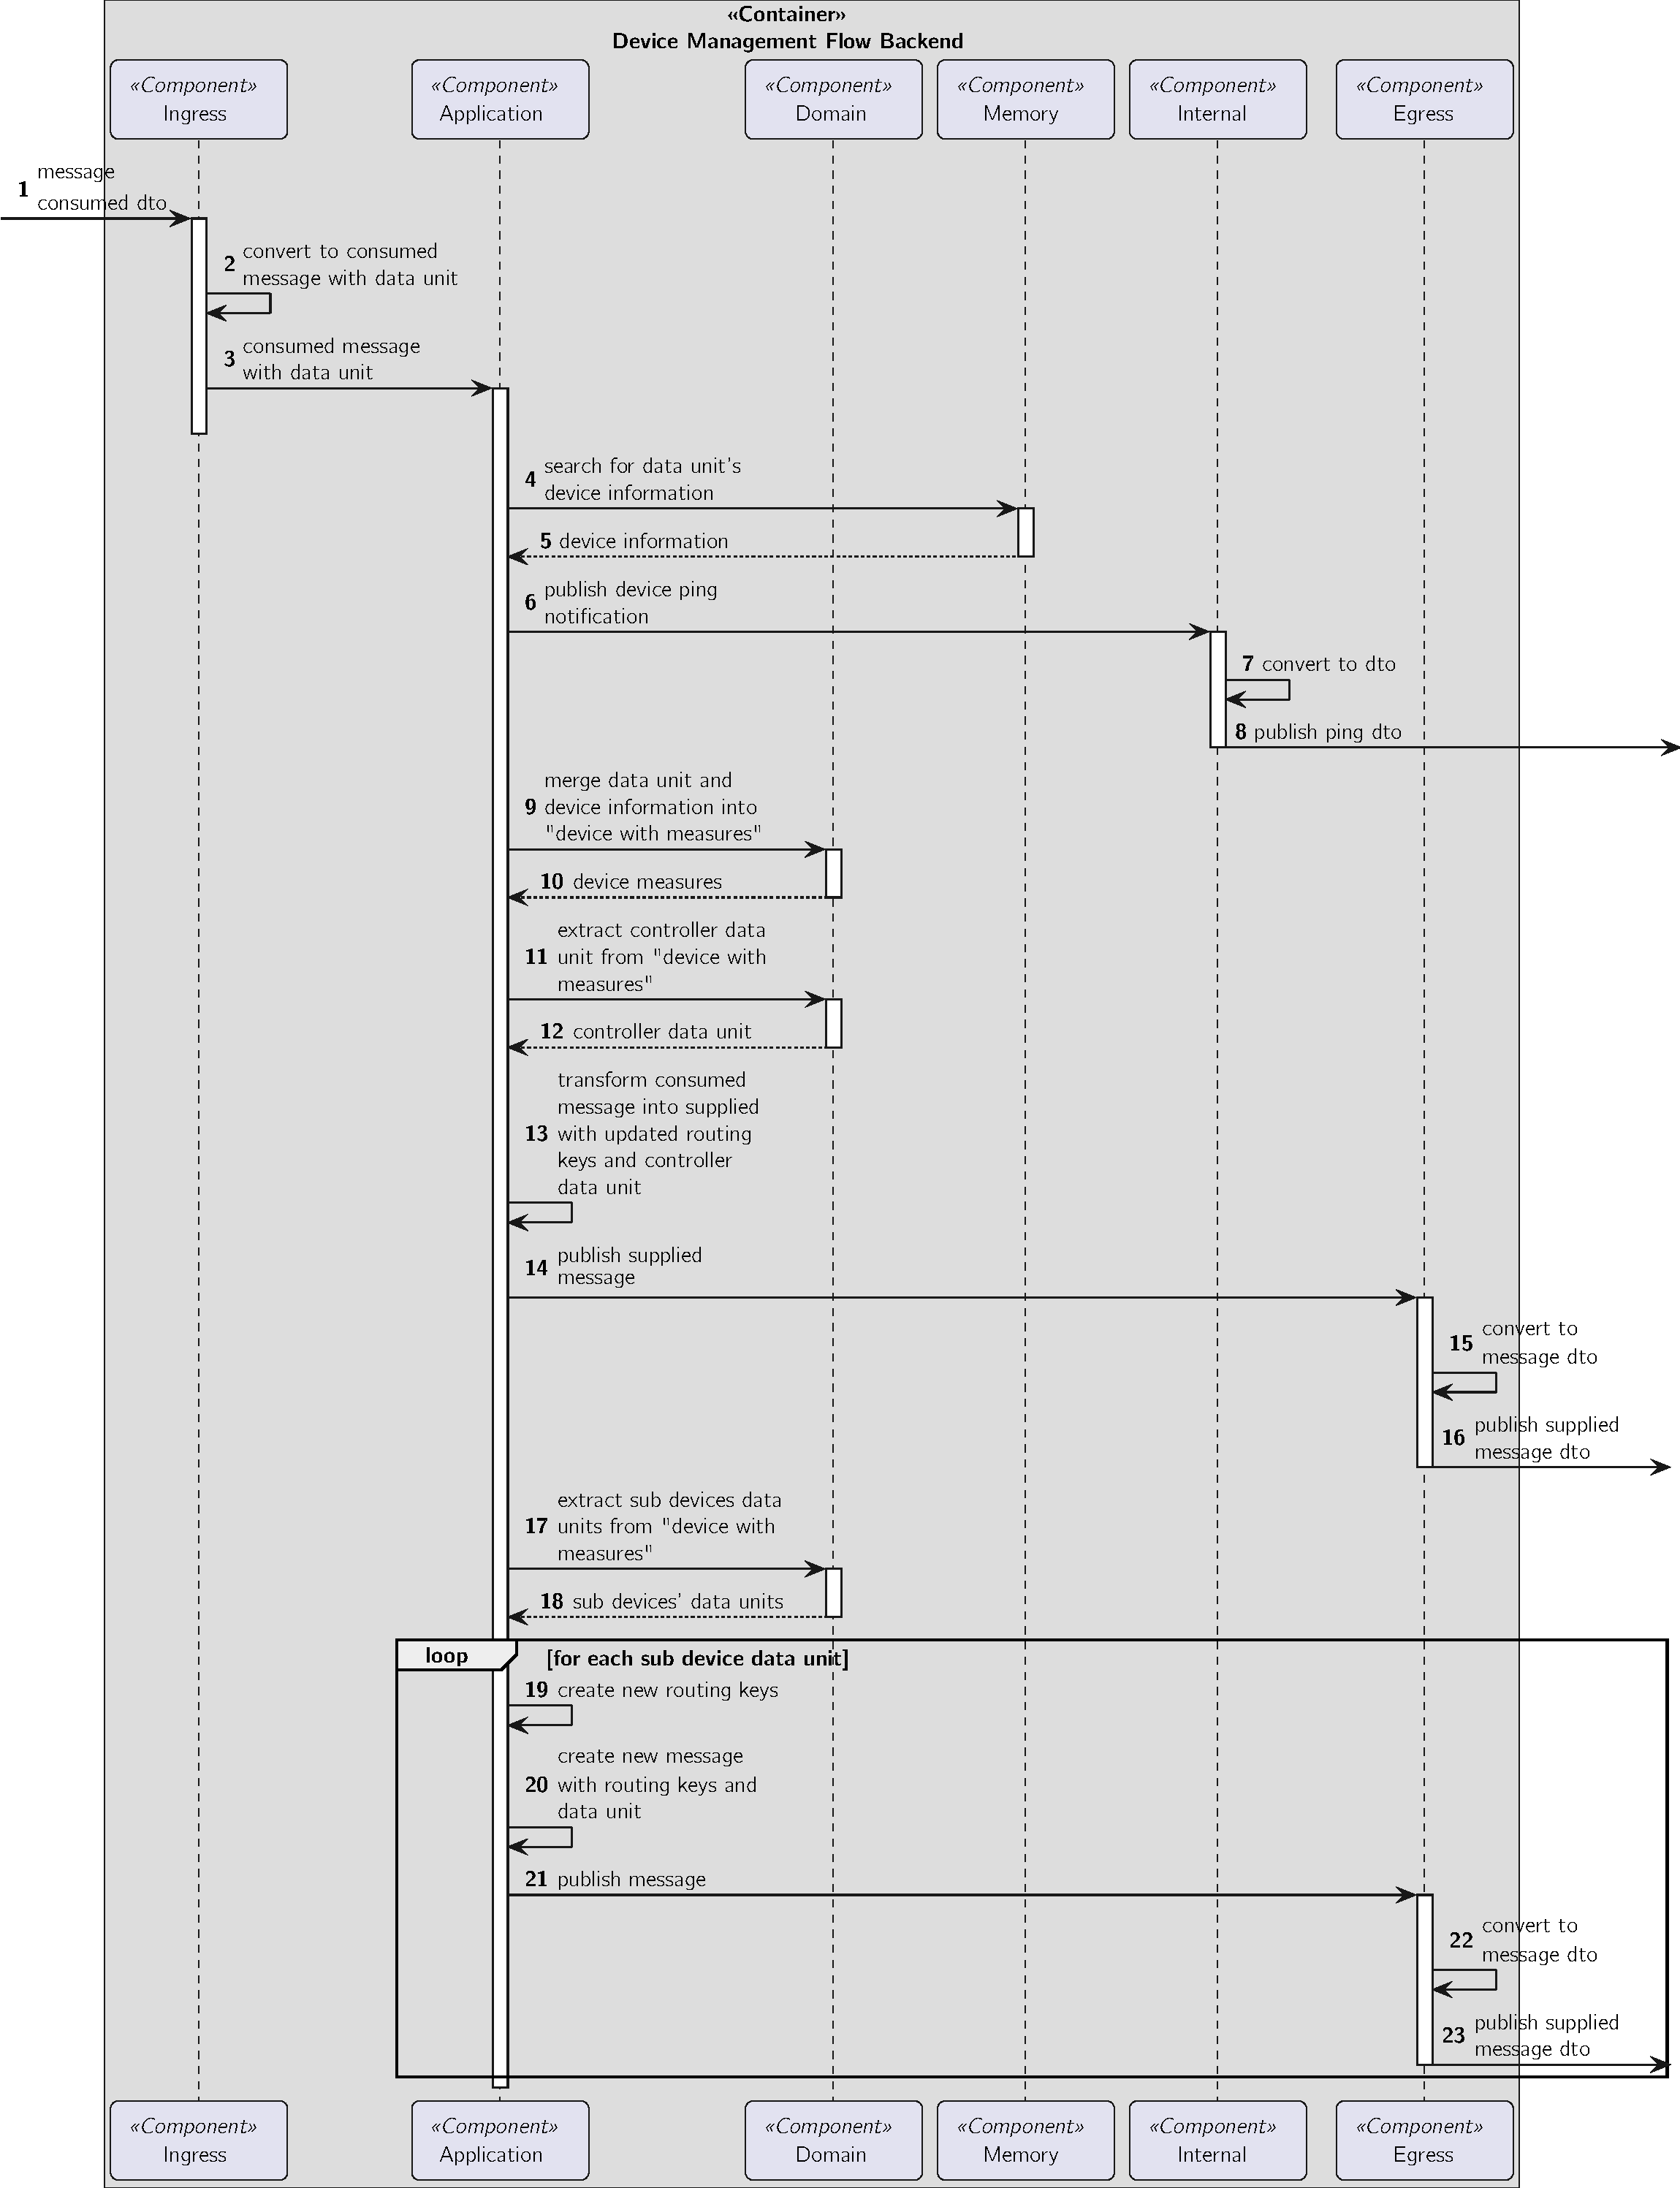
\includegraphics[page=1,width=\columnwidth]{assets/diagrams/design/architectural/level3/process/device-management-flow-backend.pdf}
   \caption[Process Data Unit in Device Management Flow Backend - Component Level - Process View Diagram]{Process Data Unit in Device Management Flow Backend - Component Level - Process View Diagram}
   \label{fig:design:architecture:platform:component:process:diagram:device}
\end{figure}

As presented in the diagram:

\begin{itemize}
   \item As soon as the message dto arrives, it is mapped to the \textit{iot-core} data unit model - step \textbf{2} - this model is used inside every Data Flow container. Before publishing the data unit it is mapped to the dto once again - step \textbf{15} and \textbf{22}. This conversion happens with any other event published and consumed in the system;
   \item If the device information is found, a \textit{ping} notification for that device is sent - steps \textbf{6} to \textbf{8}, otherwise an \textit{unknown} notification would be sent and the container would store the data unit in the Memory component and process it when possible;
   \item For each sub device of the controller, a new data unit with that device measures is published in the system - steps \textbf{19} to \textbf{23};
\end{itemize}

Next, the process of deploying draft rule scenarios is described.
Draft scenarios exist since adding, removing or changing a rule scenario in Alert Dispatcher Backend requires the entire data set to be removed. This procedure can lead to alerts not being dispatched. The next diagram, Figure~\ref{fig:design:architecture:platform:component:process:diagram:rule}, tackles this concern.

\begin{figure}[H]
   \centering
   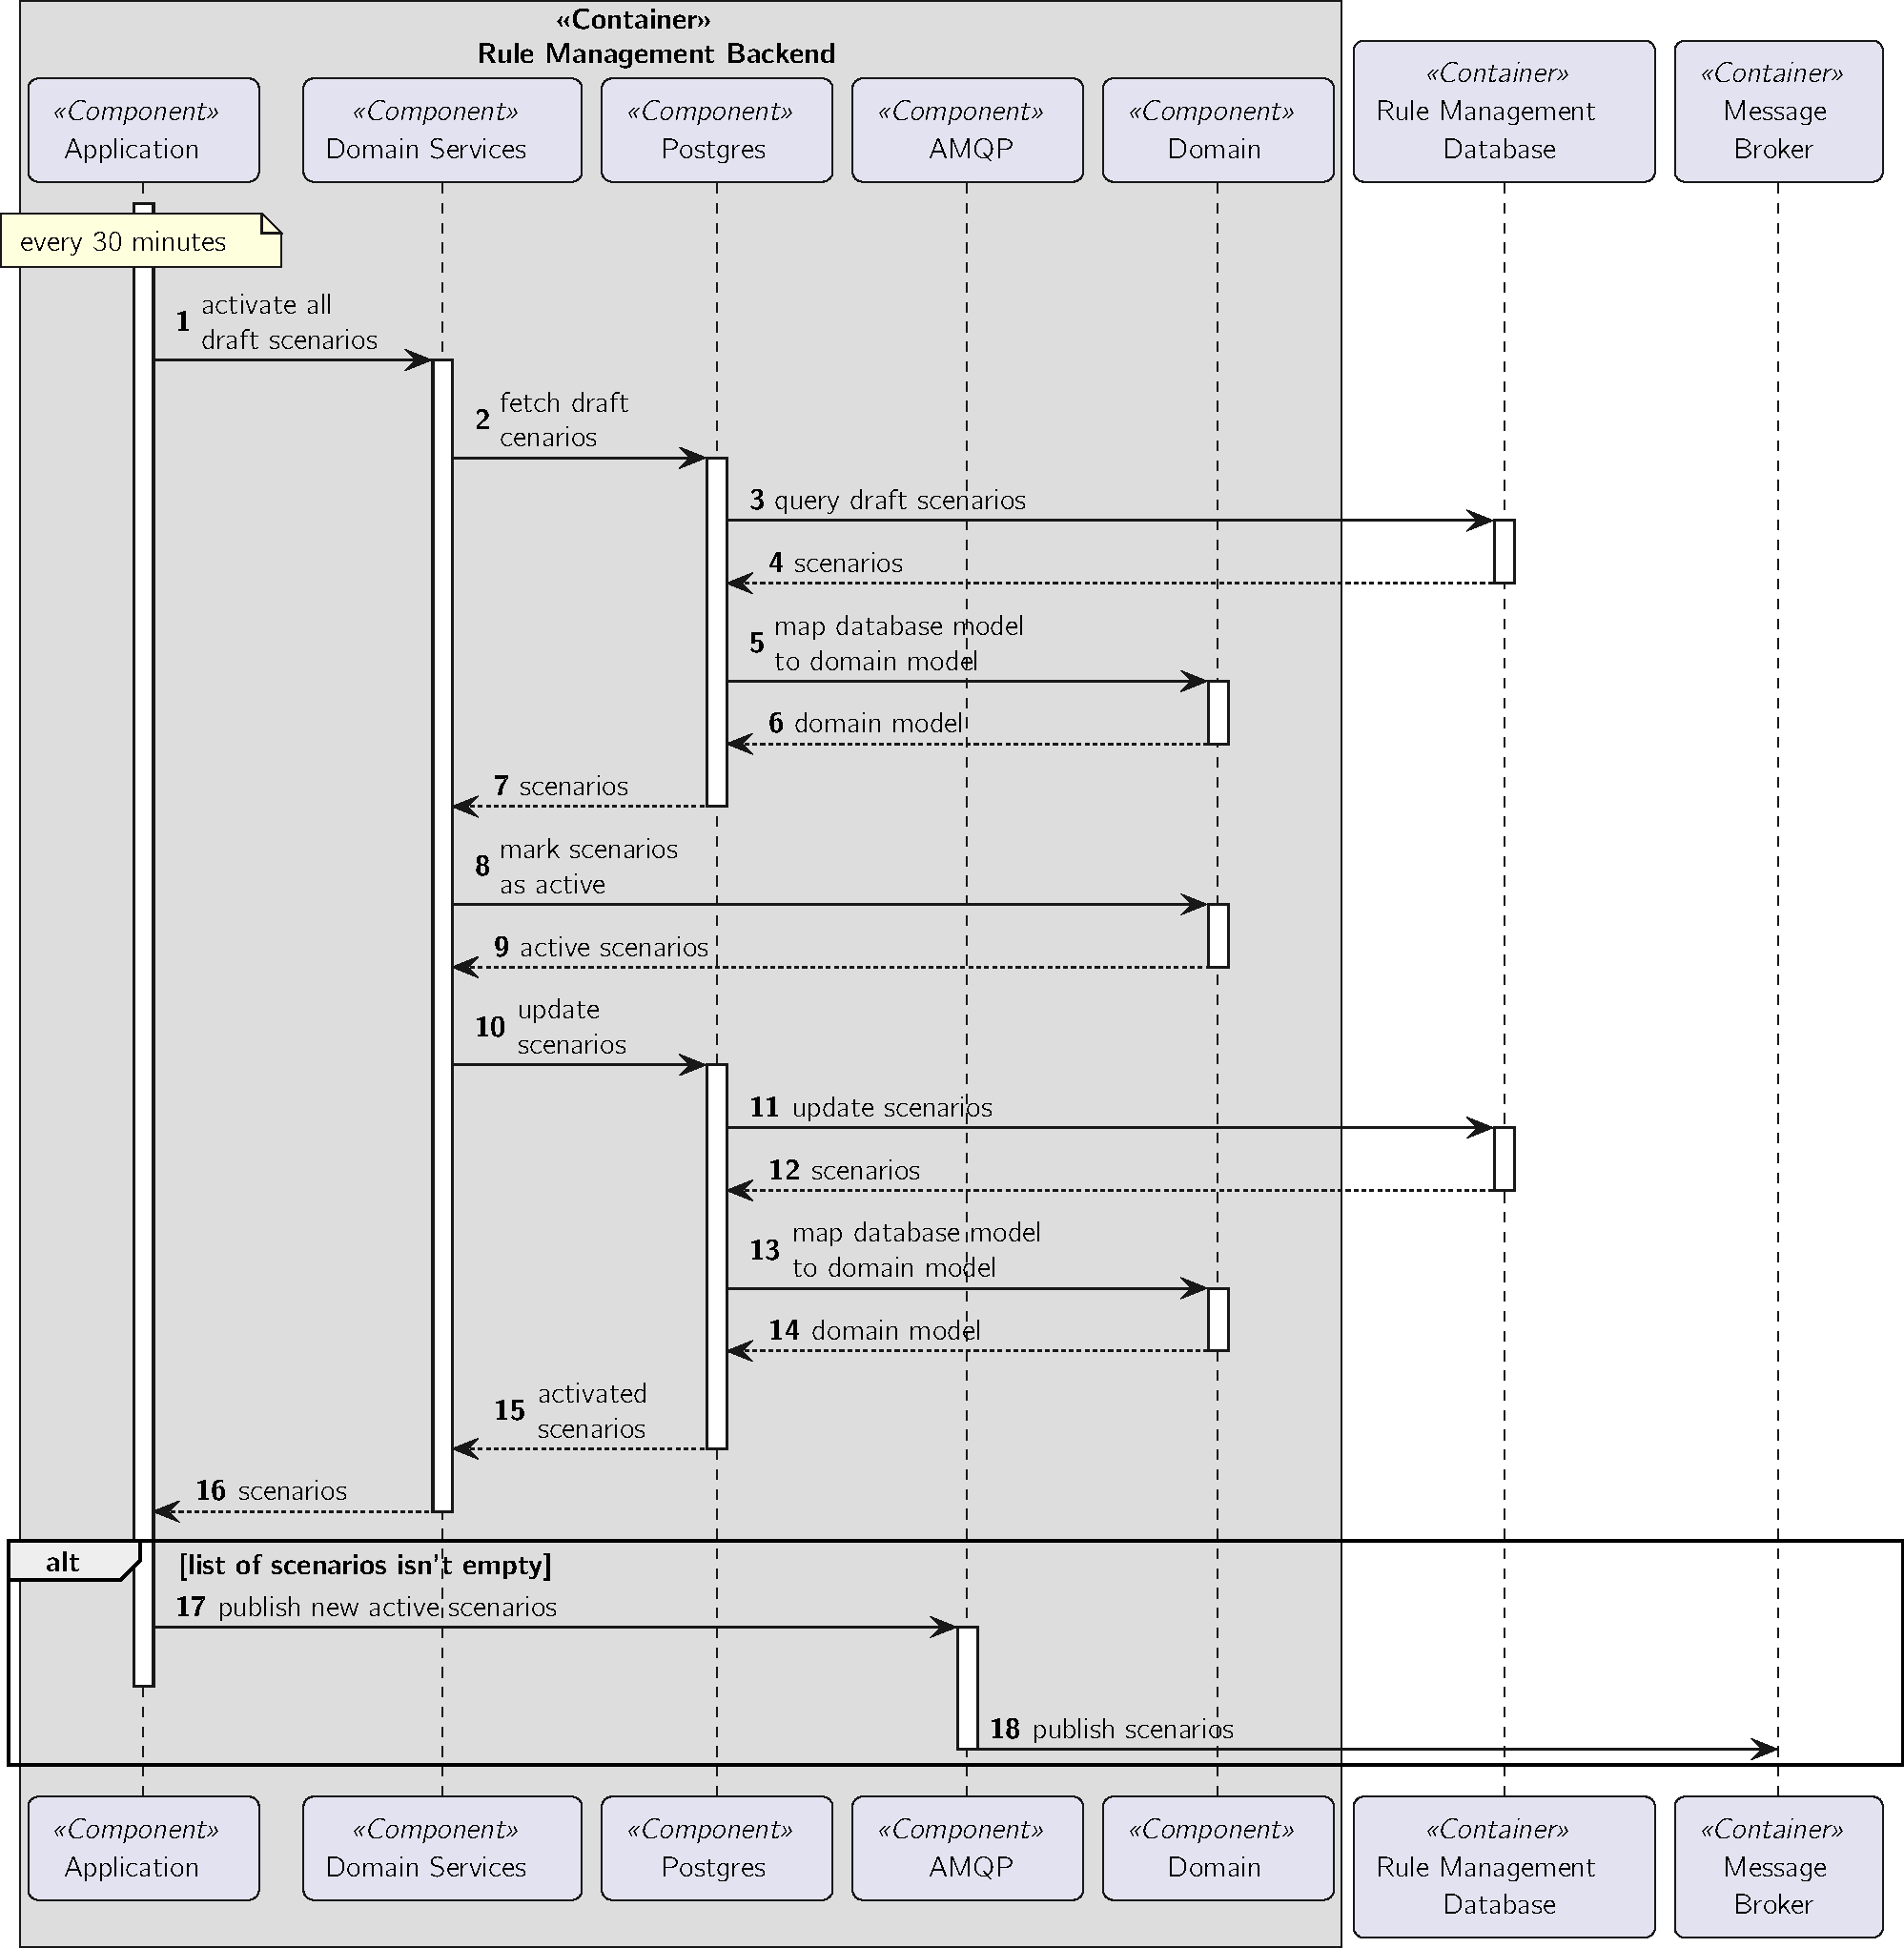
\includegraphics[page=1,width=\columnwidth]{assets/diagrams/design/architectural/level3/process/rule-management-backend.pdf}
   \caption[Deploy Draft Rule Scenarios - Component Level - Process View Diagram]{Deploy Draft Rule Scenarios - Component Level - Process View Diagram}
   \label{fig:design:architecture:platform:component:process:diagram:rule}
\end{figure}

As seen in the diagram, to mitigate the number of lost alerts, new rule scenarios are published at best every 30 minutes - step \textbf{1} - and only if any change was made - step \textbf{17} and \textbf{18}.

\section{Components Level - Implementation View}
\label{par:design:architecture:platform:components:development}

The implementation view of each container can also be condensate in the same 3 distinct types presented in the Section \nameref{par:design:architecture:platform:components:logical}.

The next diagrams, Figure~\ref{fig:design:architecture:platform:component:development:diagram:decoder}, Figure~\ref{fig:design:architecture:platform:component:development:diagram:device} and Figure~\ref{fig:design:architecture:platform:component:development:diagram:ownership} describe this view at the components level.

\begin{figure}[H]
   \centering
   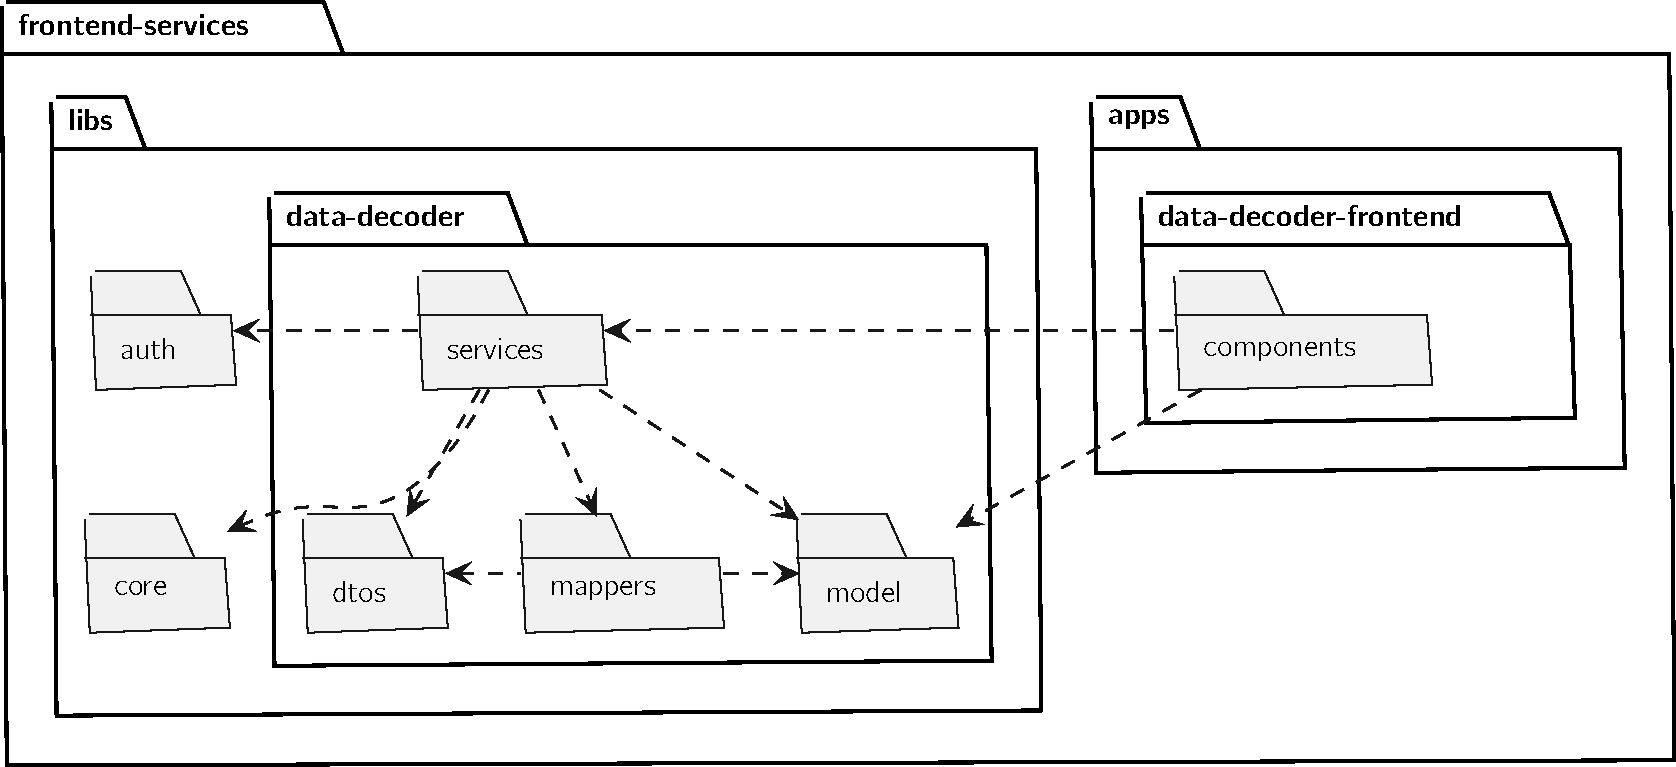
\includegraphics[page=1,width=\columnwidth]{assets/diagrams/design/architectural/level3/development/data-decoder-frontend.pdf}
   \caption[Data Decoder Frontend - Component Level - Implementation View Diagram]{Data Decoder Frontend - Component Level - Implementation View Diagram}
   \label{fig:design:architecture:platform:component:development:diagram:decoder}
\end{figure}

The packages presented correspond to the components described in the logical view (Figure~\ref{fig:design:architecture:platform:component:logical:diagram:decoder}). Since the names given in both views are different, the following list maps the logical view into the implementation view:

\begin{itemize}
   \item \textit{components} package corresponds to the \textit{Presentation} component;
   \item \textit{auth} package corresponds to the \textit{Auth} component;
   \item \textit{core} package corresponds to the \textit{Utils} component;
   \item \textit{dtos} package corresponds to the \textit{DTOS} component;
   \item \textit{mappers} package corresponds to the \textit{Mappers} component;
   \item \textit{model} package corresponds to the \textit{Model} component;
   \item \textit{services} package corresponds to the \textit{Services} component.
\end{itemize}

\begin{figure}[H]
   \centering
   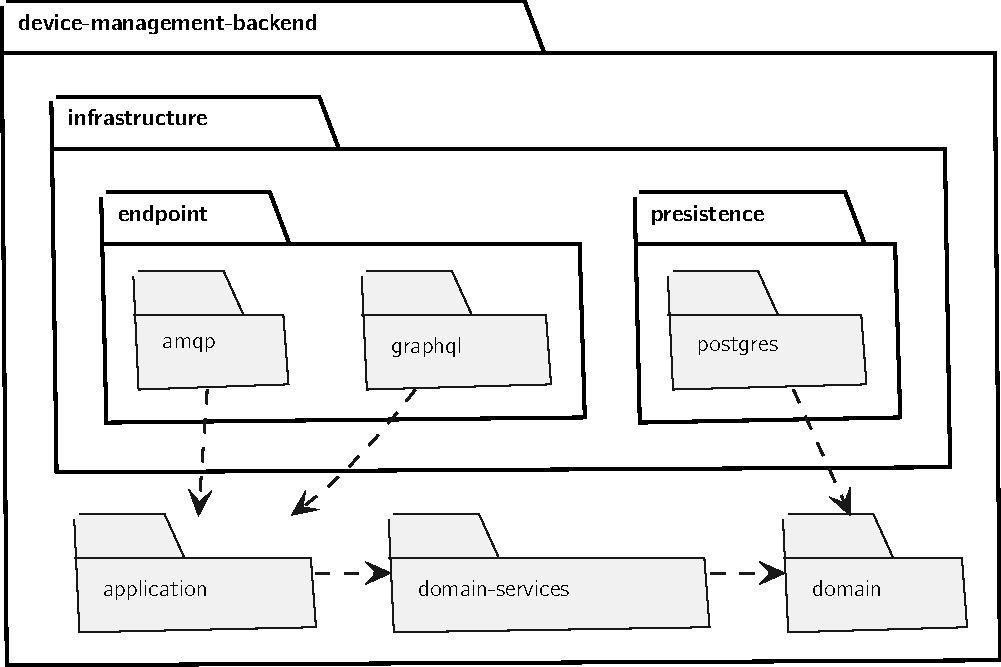
\includegraphics[page=1,width=0.8\columnwidth]{assets/diagrams/design/architectural/level3/development/device-management-backend.pdf}
   \caption[Device Management Backend - Component Level - Implementation View Diagram]{Device Management Backend - Component Level - Implementation View Diagram}
   \label{fig:design:architecture:platform:component:development:diagram:device}
\end{figure}

The packages presented correspond to the components described in the logical view (Figure~\ref{fig:design:architecture:platform:component:logical:diagram:device}). The names given in both views differ only on the case used.

\begin{figure}[H]
   \centering
   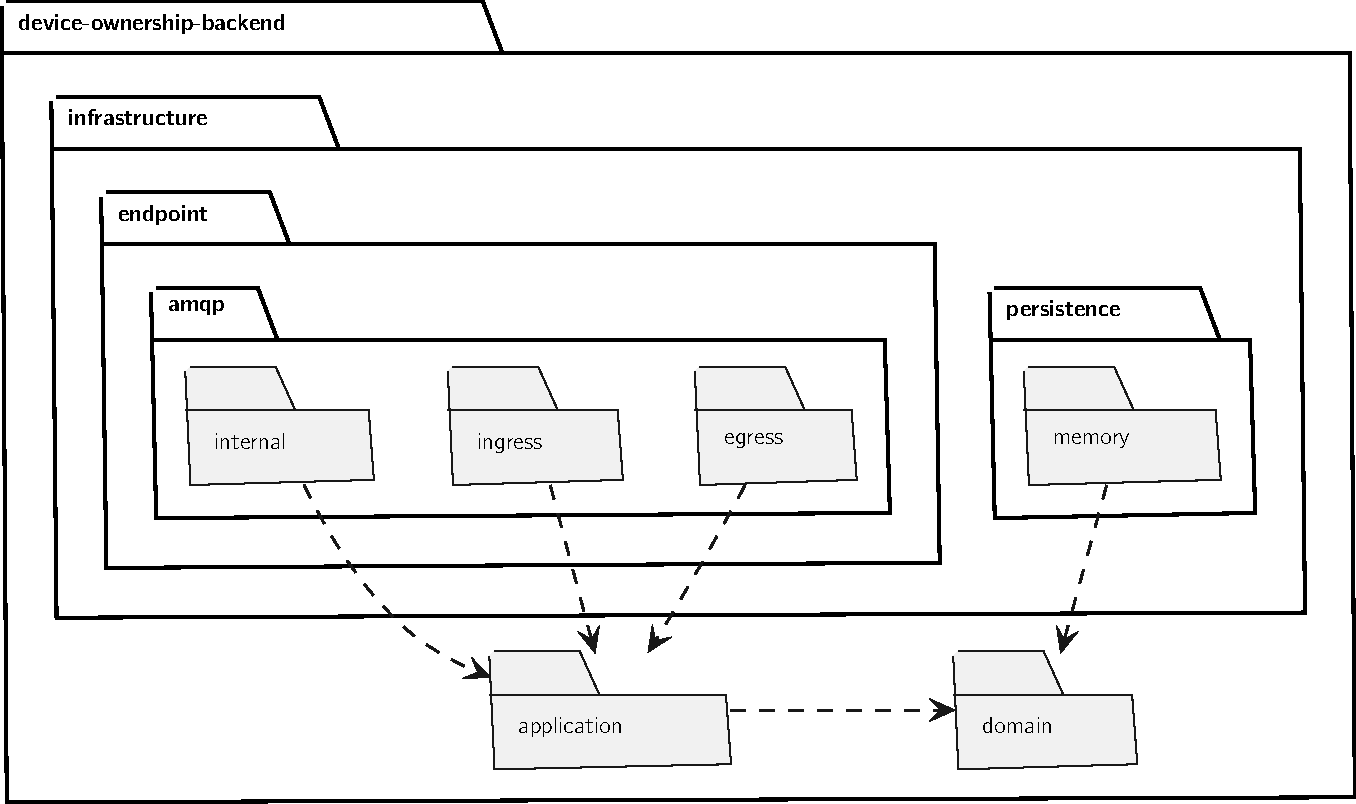
\includegraphics[page=1,width=0.8\columnwidth]{assets/diagrams/design/architectural/level3/development/device-ownership-backend.pdf}
   \caption[Device Ownership Backend - Component Level - Implementation View Diagram]{Device Ownership Backend - Component Level - Implementation View Diagram}
   \label{fig:design:architecture:platform:component:development:diagram:ownership}
\end{figure}

The packages presented correspond to the components described in the logical view (Figure~\ref{fig:design:architecture:platform:component:logical:diagram:ownership}). The names given in both views differ only on the case used.
